\chapter{Computing in DUNE}
\label{ch:exec-comp}

\fixme{Heidi, this outline may be overkill for the exec summary; it may be a good structure for the computing CDR volume, then pared down for inclusion here. My 2 cents! -Anne}
%%%%%%%%%%%%%%%%%%%%%%%%%%%%%%%%%%%%%%%%%%%%%%%%%%%%%%%%%%%
%\section{To remove: just examples}
%\label{sec:exec-comp-1}
%
%Sample figure to copy and edit, Figure~\ref{fig:map}:
%
%\begin{dunefigure}[DUNE collaboration global map]{fig:mhexec}{The international DUNE
%collaboration. Countries with DUNE membership are shown in orange.}
%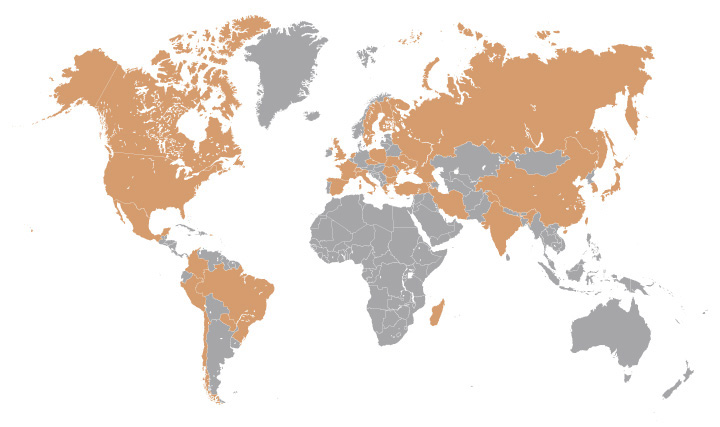
\includegraphics[width=0.9\textwidth]{global-retouched.jpg}  
%\label{fig:map}
%\end{dunefigure}
%
%Sample table to copy and edit, Table~\ref{tab:execosctable}:
%
%\begin{dunetable}[Required exposures to reach oscillation physics
%  milestones]{lcc}{tab:execosctable}{The exposure in mass (kt) $\times$ proton beam power
%    (MW) $\times$ time (years) and calendar years assuming the staging plan described in this chapter needed to reach certain oscillation physics
%    milestones. The numbers are for normal hierarchy using the NuFit 2016 best fit values of the known oscillation parameters.  }
%Physics milestone & Exposure  & Exposure \\ \rowtitlestyle
%  & (\ktMWyr{}) & (years)  \\ \toprowrule 
%  $1^\circ$ $\theta_{23}$ resolution ($\theta_{23} = 42^\circ$) & 29  &  1\\ \colhline
%  CPV at $3\sigma$ ($\delta_{\rm CP} = -\pi/2$)  & 77 &  3\\ \colhline
%  \dword{mh} at  $5\sigma$ (worst point) & 209 & 6 \\ \colhline
%  $10^\circ$ $\delta_{\rm CP}$ resolution ($\delta_{\rm CP} = 0$) & 252 & %5 
%  6.5 \\ \colhline
%  ($\sin^2 2 \theta_{13} = 0.084 \pm 0.003$) &  &  \\  
%\end{dunetable}
%
%%%%%%%%%%%%%%%%%%%%%%%%%%%%%%%%%%%%%%%%
\section{Executive Summary}		
\label{ch:exec-comp-es}







The DUNE long baseline neutrino oscillation collaboration consists of 178 institutions from 32 countries, including 15 European nations and \dword{cern}. The experiment is in preparation now with commissioning of the first module expected over the period 2024-2026 and a long data taking run with 4 modules expected from 2026-2036 and beyond.  An active prototyping program is already in place with a short test beam run with a 700T, 15,360 channel prototype of single-phase readout at the neutrino platform \dword{cern} in late 2018 and tests of a similar sized dual-phase detector scheduled for mid-2019.   The DUNE experiment has already  benefited greatly from these initial tests.  The collaboration has recently formed a formal Computing Consortium, with significant participation by European Institutions and interest from groups in Asia to work on common software and computing development and to formalize resource contributions.

The consortium resource model benefits from existing Grid and \dshort{wlcg} infrastructure developed for the LHC.  DUNE, through  the ProtoDUNE-SP effort, is already using global resources for simulation and the analysis of ProtoDUNE-SP data.  Multiple European sites are part of this resource pool and are making significant contributions to the ProtoDUNE single and dual phase programs.  We expect this global computing consortium to grow and evolve as we move towards data from the full DUNE detectors in the middle of the next decade.

The DUNE science program is expected to produce raw data volumes similar in scale to the data volumes that current LHC Run-2 experiments have already recorded.  Baseline predictions for the DUNE data, dependent on actual detector performance and noise levels, are 30-60 PB of raw data per year.  These data, with simulations and derived analysis samples, need to be available to all collaborating institutions.  We anticipate that institutions worldwide will play an important role both as contributors and end-users of storage and CPU resources for DUNE.

To enable these resource contributions in cooperation with the LHC and other communities, we plan to utilize common computing layers for infrastructure access and use common tools to ease integration of facilities with both the DUNE and LHC computing ecosystems.  For example, we plan to utilize common data storage methodologies to establish large highly available data lakes worldwide  and to collaborate with the broader HEP community in developing other common tools.

The 2018 test beam run of protoDUNE Single-Phase (SP) was a valuable live test of this model.  The ProtoDUNE Single Phase detector at CERN produced raw data at rates of up to $\sim\,\SI{2}{GB/s}$ of data.  These data were stored on tape at CERN and Fermilab and replicated at sites in the UK and Czech Republic.  In total 1.8 PB of raw data were produced during the test beam run. 
This prototype run has been extremely beneficial in exercising the existing computing infrastructure and in building a team of interested institutions.

HEP has considerable infrastructure in place for international computing collaboration thanks to the LHC program.  Other large experiments -- LSST, SKA, DUNE and HyperK -- will be coming on board over the next decade.   DUNE's strategy is to work with the global community to maximize the use of common tools for data movement and storage, job control and monitoring, accounting and authentication.   All large-scale experiments will encounter similar issues and worldwide cooperation on common tools is the most cost-effective way to proceed. For example, in collaboration with the Fermilab, CERN and the UK groups, we are investigating the use of Rucio as our primary data manager.

In addition to traditional HEP computational strategies, DUNE's data consists of simple but very large 2D data objects which share many characteristics with astrophysical images.  This presents opportunities to use current advances in machine learning and pattern recognition as a frontier user of High Performance Computing facilities capable of massively parallel processing.  We share this problem, and propose to share solutions, with the other Liquid Argon experiments - ArgoNeut, MicroBooNE, SBND and ICARUS.  We have already benefited greatly from prior work and plan to contribute cooperatively.

In summary, DUNE's computing strategy is to be {\bf global}, working with partners worldwide, and {\bf collaborative}, as almost all of the computational challenges we face are faced by similar experiments. 
 


%%%%%%%%%%%%%%%%%%%%%%%%%%%%%%%%%%%%%%%%
\section{Overview}		
\label{ch:exec-comp-ovr}
The main goal of the computing effort is to facilitate the acquisition, processing and analysis of data and simulations from the DUNE experiment across the many physics drivers for the experiment in a cost effective way. Computing and Software provides the bridge between the real-time online systems of the DUNE/LBNF hardware and the physics groups who develop high-level algorithms and perform data analysis. S+C works with collaborating institutions to idify CPU and storage resources and to support basic software infrastructure such as software frameworks, data catalogs, database infrastructure and code distributions systems. 

The Consortium is currently working with national agencies and major laboratories to negotiate CPU and storage provision for the near term protoDUNE runs and development of the full DUNE computing model and is starting the process of evaluating major software infrastructure systems such as workload management, emphasizing collaboration and reuse of existing systems. 

Our initial assessment of needs indicates that data rates and CPU needs for DUNE are significantly less than those for the large LHC experiments but that the extremely large size of individual DUNE events presents unique technical challenges that will require substantial effort to address. 


\subsection{Data types and volumes}
Maximum raw data volumes from the detectors are reasonably easy to estimate, as a product of trigger rate, number of channels, \# of time slices/channel,  size for each ADC readout and compression. However, those data sizes would be well beyond the ability of any system to handle. Thus decisions must be made about what to keep and what not to keep. Those decisions are the purview of the collaboration scientists and the data acquisition design with feedback from computing on what is possible.  The ProtoDUNE experience has provided invaluable information to feed back to the experiment design. 




\subsubsection{Far detector data volumes}

The computing model needs to be able to handle a wide range of data inputs from the far detectors, as documented in more detail in~\cite{bib:docdb9240}. \fixme{add to bib}

\begin{itemize}
\item Supernova triggers which would have an uncompressed size of 138 TB for a 30 second readout of all channels in a 4-module single-phase detector at a likely rate of 1/month.  
\item Beam neutrino interactions within a single detector module with an uncompressed size of $\approx$ 6.2 GB at a rate of up to 1 Hz
\item Atmospheric neutrino interactions, nucleon decay and other lower energy processes confined to a subset of a detector module with a low threshold largely driven by radiological backgrounds.
\item Cosmic ray and rock muons at a rate of around 4,500/day/module.
\item Other calibration systems 
\end{itemize}

The estimates in docdb-9240, with conservative estimates for increased needs for low level data taking during commissioning, have led to a negotiated upper limit of 30 PB/year data volume as a standard for both the trigger and data acquisition and computing groups to work towards. 


\begin{dunetable}[Useful quantities for computing estimates]{lrll}{tab:exec-comp-bigpicture}{Useful quantities for computing estimates}
Quantity&Value&Units&Explanation\\ \toprowrule
{\bf Far Detector Beam:} & & &\\ \colhline
Single APA readout &41.5& MB& Uncompressed 5.4 ms\\ \colhline
APAs per module& 150& &\\ \colhline
Full module readout &6.22&  GB& Uncompressed 5.4 ms\\ \colhline
Beam rep. rate&\beamreprate& Hz&Untriggered\\ \colhline
CPU time/event&600-1,200&sec&from MC/ProtoDUNE\\ \colhline
Memory footprint&2-4&GB&ProtoDUNE experience\\ \colhline
{\bf Supernova:} & & & \\ \colhline
Single channel readout &90.0&MB& Uncompressed 30 s\\ \colhline
Four module readout&138.2& TB& Uncompressed 30 s\\ \colhline
Trigger rate&1 & per month&(assumption)\\ 
%Yearly rates nd
%Reduction with roi.  
%CPU time/ event for reconstruction
%Reduction for analysis
%Users 
\end{dunetable}

\subsubsection{Near Detector data volumes}
In addition, a near detector of reasonable size will have multiple neutrino interactions/beam spill leading to a need to read out at the full beam rate of 0.8-1.2 Hz.
The near detector will have fewer channels and better signal/noise discrimination but much higher readout rates.  While the details of the detector design are still unknown, we assume data volumes of similar size to the far detector (30PB/year) in our planning.

\subsubsection{Simulation}
The bulk of data collected is likely to be backgrounds, with real high energy events in the far detector numbering in the thousands/year, not millions. Thus the size of simulation samples is likely to be less than that of the raw data.  Lower energy events are either very rare or can be simulated in sub-volumes of the whole detector.  As a result, while simulation will be an important part of the experiment, it is not expected to dominate data volumes as it does in many experiments.  



\section{ProtoDUNE-SP as an example}		
\label{ch:exec-comp-proto-SP}
The first protoDUNE single phase run at CERN in late 2018 has already led to a small-scale test of a global computing model.  In the following we will describe the protoDUNE data design and the lessons learned from our experience. Much of this carries over into planning for full far-detector operations. 

\subsection{Introduction}

The protoDUNE Single Phase detector ran at CERN in the np04 beamline from September to November of 2018. Since then, studies with cosmic rays have continued. Prior to that run there were several data challenges at high rate to validate the data transfer mechanisms. 

The first phase of operations was commissioning of the detector readout systems while the argon reached full purity.  Data were taken with cosmic rays and beam during the commissioning period.  



\subsection{Data volumes}
The single-phase protoDUNE detector consists of a \dshort{tpc} with  6 Anode Plane Assemblies (\dshort{apa}), photon detectors (\dshort{pd}s) and a Cosmic Ray Tagger (\dshort{crt}). In addition, the np04 beamline is instrumented with hodoscopes and Cerenkov counters to generate beam triggers and random readouts were done at lower rates to collect unbiased cosmic ray information. The data volume from the test beam run was dominated by readout of the \dshort{apa} planes.  Each \dshort{apa} has 2,560 channels and reads out 12 bit ADC values at 2 MHz.  During beam running, the detector was triggered on the incoming beam. The nominal readout window during beam running was  3 ms to match the drift time at the full voltage of 180 kV that was maintained for most of the run.  The total size of the \dshort{tpc} data without compression was thus 138 MB/event.  Compression was implemented before the October beam physics run, lowering the total size per event from around 180 MB to 75 MB.  

\begin{dunetable}[Data volumes]{lrr}{tab:exec-comp-pd-volumes}{Data volumes  recorded by ProtoDUNE-SP}
Type  & Events & Size\\ %\rowtitlestyle
Raw Beam&8.08 M& 520 TB \\
Raw Cosmics&3.46 M& 271 TB\\
Commissioning&3.86 M& 388 TB\\
Pre-commissioning&13.89 M&641 TB\\
\end{dunetable}

Events were written out in raw files of size 8 GB with each containing of order 100 events. The beam was live for two 4.5 s spills every 32 s beam cycle and data were taken at peak rates of up to 50 Hz (typically 25 Hz) leading to compressed DC rates out of the detector of 400-800MB/sec.  Each beam cycle could therefore produce 1-4  8 GB output files.  In earlier running with uncompressed data, and during an April data challenge, transfer rates of up to 2GB/s were demonstrated over substantial periods. 

Beam stopped in November 12 but cosmic ray studies of the detector continue, some with an increase time window of 7.5 ms to collect more complete tracks/readout.  This raises the compressed event size to around 170 MB.

\subsection{ProtoDUNE-SP data streams}
The protoDUNE-SP data consist of multiple sources in addition to the TPC data. One of the major challenges for the offline computing systems is merging of these multiple streams into a coherent whole for analysis. 

\begin{dunetable}[Data sources]{lrr}{tab:exec-comp-pd-sources}{Data sources  }
Type & indexed by & destination\\
TPC  & run/event & event data\\
Photon Detector data & run/event & event data\\
Cosmic Ray Tagger & run/event & event data\\
Beamline devices & time-stamp & beam database\\
Detector conditions & time-stamp & slow controls database\\
DAQ configuration & run & files/elisa logbook\\
Run quality & run & human generated spreadsheets\\
Data quality & run/event/time & Data Quality web application\\
File metadata & file & sam file database\\
\end{dunetable}

Information about the detector conditions, \dword{daq} configuration and run quality is spread across a number of sources and must be collected and then boiled down into the quantities relevant for offline data analysis.  For example, the Slow Controls system logs detector conditions continually.  Offline analysis needs to know about these data with coarser granularity and then have algorithms capable of using that information. A full conditions database transfer mechanism is being developed but was not available during the run.  As a result, with the exception of beamline information, coarse information is currently added to the \dword{sam} file catalog run by run to allow files with given operating conditions to be easily identified and retrieved. Beam data is stored in the \dword{ifbeam}
database and connected to event data via time stamps.

\section{Reconstruction of protoDUNE-SP data}
Thanks to substantial previous effort by the 35T prototype, \dword{microboone} and the liquid argon community, high quality algorithms were already in place to reconstruct the data.  As a result, a first pass reconstruction of the protoDUNE-SP data with beam triggers was completed by early December, less than a month after the end of data taking.

\subsection{Reconstruction}

The TPC data read from the protoDUNE detector includes a waveform for
each of 15360 channels. Each waveform is the output of a 16-bit ADC sampling
at 2~MHz the output voltage of a charge-sensitive amplifier connected to one of
the TPC Wires. 
%%The most interesting contribution to these signals is the
%charge on the wire induced by the motion of electrons in the TPC.
%There are also deliberate voltage offsets to put the signal in the amplifier
%and ADC ranges and there is noise from the electronics (jitter and pickup)
%and wire motion. Finally, each ADC channel has response nonlinearity and
%distortions.

The electrons produced in the \dword{tpc} volume drift % away from a cathode plane
toward three planes of anode wires with voltage bias such that the electrons
pass through the first two planes (called induction planes) and are collected
on the last (collection plane).
The signal induced on the collection plane wires is unipolar 
and the pedestal-subtracted area of the signal is roughly proportional to the
charge collected on that wire.
The signals on the induction wires are bipolar: first a positive signal is produced as
electrons approach the plane and then negative as they move away.
%The time (i.e. waveform sample) at which the signal appears provides a measure of the drift
%time which is used to deduce the drift distance.
\subsection{Data preparation}

Before pattern recognition, data from the protoDUNE detector is
unpacked and copied to a standard format (larsoft raw::RawDigit).
The same format is produced in detector simulation.
This reformatted raw data includes the waveform for each channel, an
integer in the range [0, 4095] for each of 6000-15,000 ticks.

The first step in reconstruction is data preparation with the goal of
converting each ADC waveform into a calibrated charge waveform with
signals proportional to charge (e.g. number of electrons) passing through
the anode plane area read out by its wire.
At the end of data preparation, regions of interest (ROIs), i.e. blocks of contiguous samples where
useful signals appear, are identified and the data outside these regions are discarded.

%Perhaps most important, the bipolar signals in induction wires are made unipolar.
%Also the electronics shaping is replaced with the Gaussian shaping expected in the
%next stage of processing.
%Relative channel-to-channel and absolute calibration is applied to account for the
%responses of the amplifiers and ADCs.
%And attempts are made to remove noise and mitigate ADC distortions.

The sequence is described more fully in docdb-12349\cite{ref:docdb12349} but is summarized here:

\begin{enumerate}
\item Each waveform is unpacked into integers.
\item Pedestals are determined per event/per channel from the most common ADC value. 
\item Pedestals and calibrations are applied. %\label{local:ped}
\item Bad channels, sticky bits and other know hardware problems are corrected or removed.
\item Signal undershoot that creates a long negative tail is removed. 
\item The waveforms  are deconvoluted.  In the first processing this was done with simple 1-D convolution for a single wire but in future the 2-D convolution described by the MicroBooNE collaboration in \cite{Adams:2018dra} will be used to eliminate cross-talk with adjacent wires.  The deconvolution Fourier transforms the waveform, applies a response function, applies a low pass filter to remove high frequency noise and then transforms back.



\item Finally regions of interest are defined where the signal exceeds a given threshold and ticks well outside the ROI are dropped, leading to significant reduction in the size of the remaining data. These data are then fed into the reconstruction algorithms for further pattern recognition. %\label{local:roi}
\end{enumerate}




\subsection{Signal processing}
Figures~\ref{fig:ch-exec-comp-chtraw}-\ref{fig:ch-exec-comp-chtroi} show how the ADC data changes during data
preparation.

\begin{figure}[t]
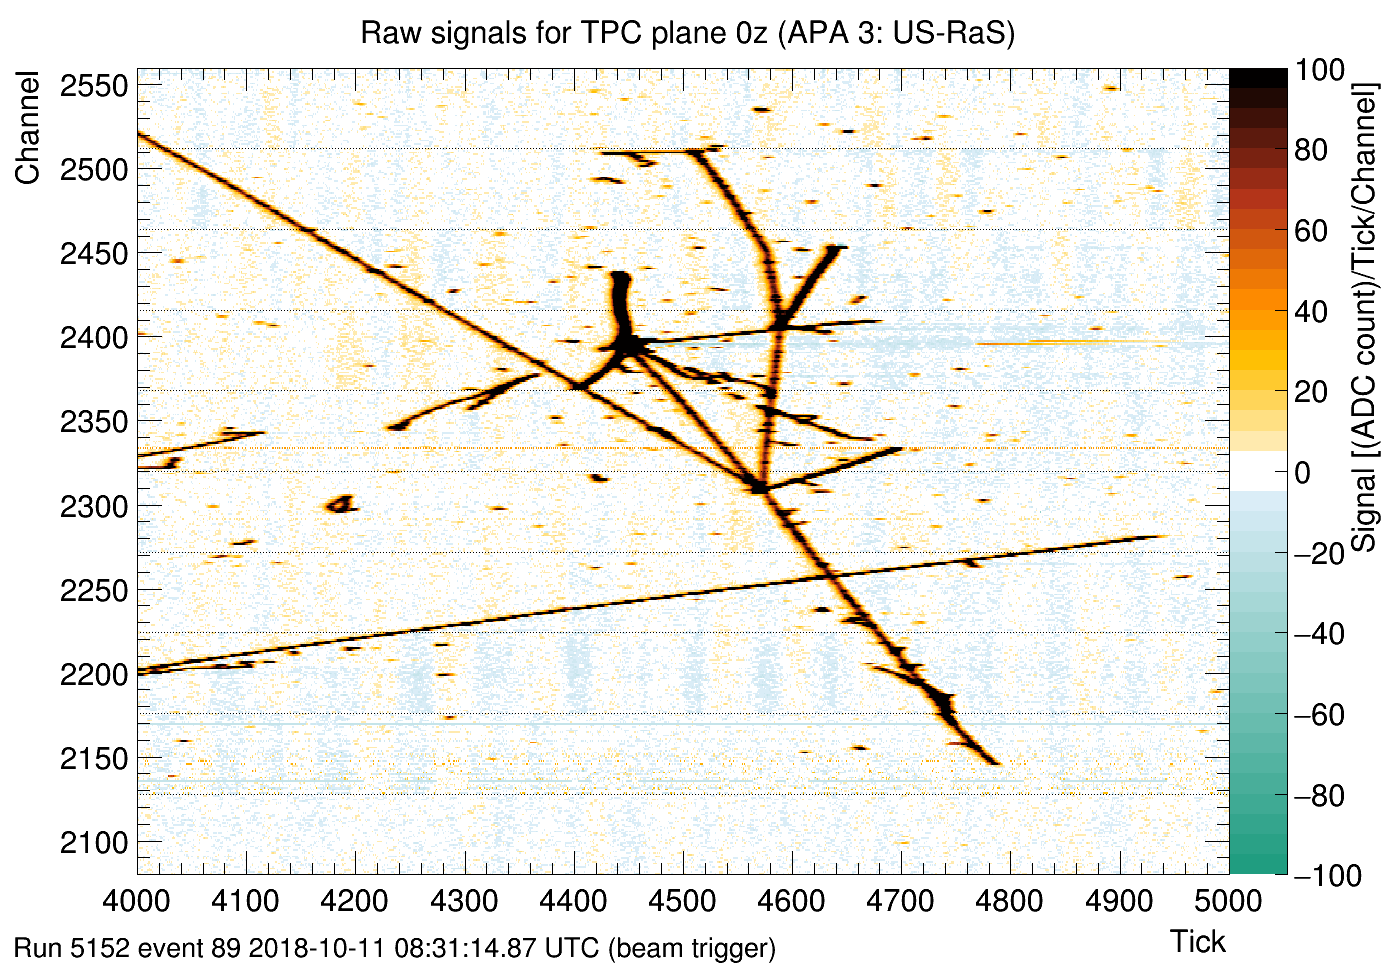
\includegraphics[width=\textwidth,angle=0]{comp-adcraw_tpp0z_run005152_evt000089.png}
\caption{
Example of pedestal-subtracted data for one of the ProtoDUNE collection wire planes.
The color scale indicates the signal strength for selected ticks in all channels
in TPC-side collection plane for APA~3 which reads out the TPC where the beam enters.
This plot is made after trivial calibration, i.e. subtracting the pedestal from the raw data.
The channels for the plane are handled by ten FEMBs and the boundaries between those
are shown with horizontal dotted lines. They are numbered 301, 302,~..., 310 going
downstream, i.e.\ from the bottom in this figure.
}
\label{fig:ch-exec-comp-chtraw}
\end{figure}




\begin{figure}[t]
  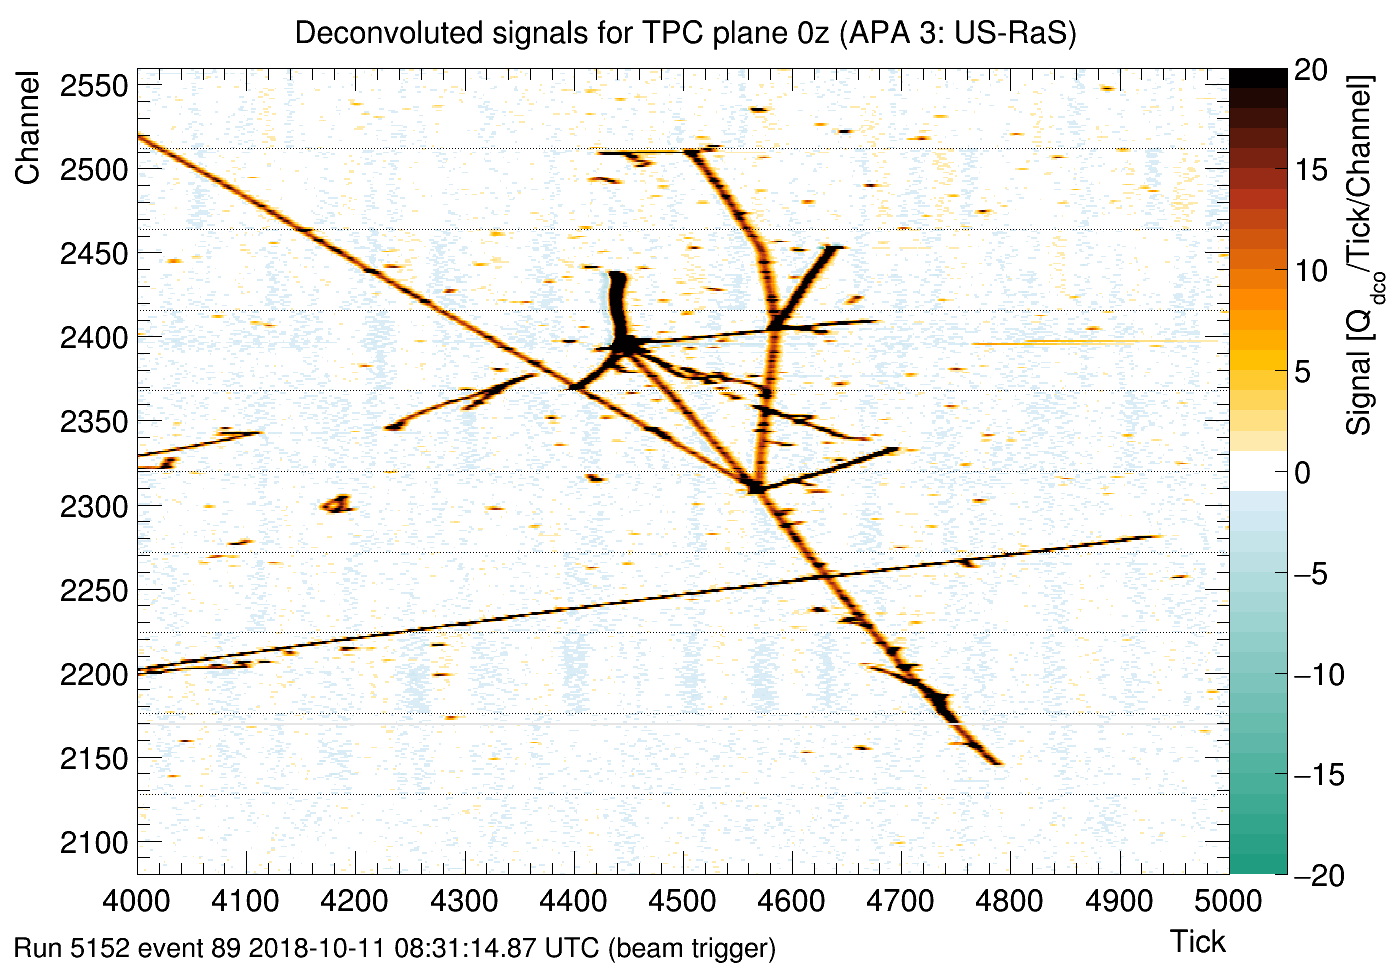
\includegraphics[width=\textwidth]{comp-adcdco_tpp0z_run005152_evt000089.png}
\caption{
Same as Fig.~\ref{fig:ch-exec-comp-chtraw} except after hit correction, tail removal and deconvolution.
}
\label{fig:ch-exec-comp-chtdco}
\end{figure}

\begin{figure}[t]
  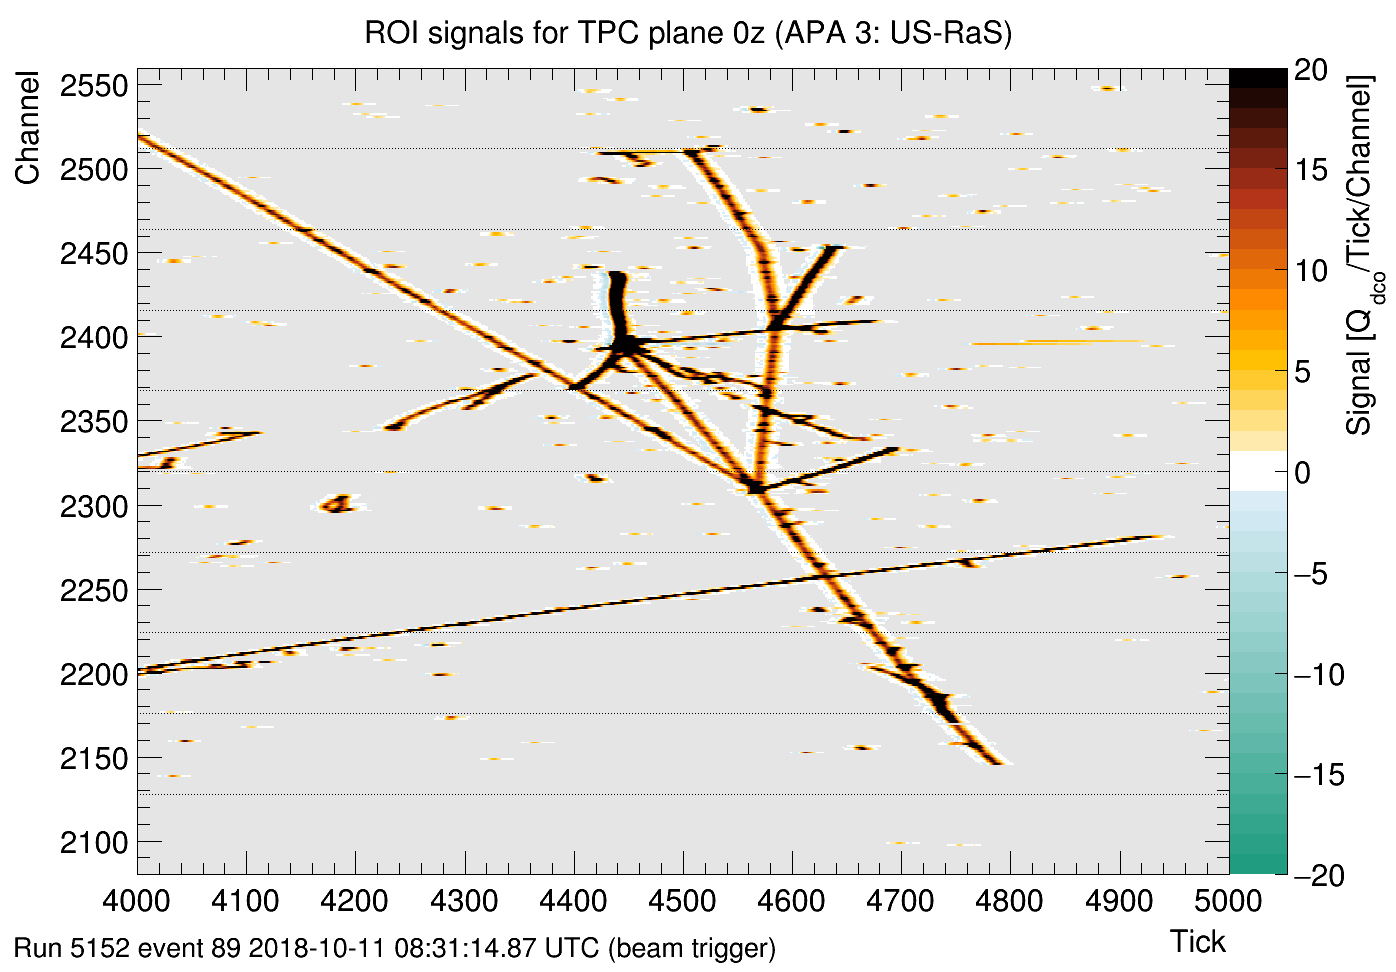
\includegraphics[width=\textwidth]{comp-adcroi_tpp0z_run005152_evt000089.png}
\caption{
Same as Fig.~\ref{fig:ch-exec-comp-chtdco} except after ROI finding. The regions in gray are
outside ROIs and excluded from the output.
}
\label{fig:ch-exec-comp-chtroi}
\end{figure}

%%%%%%%%%%%%%%%%%%%%%%%%%%%%
%\todo{Statement about timing and memory for this phase}

\subsection{Computational characteristics of data preparation and deconvolution }
Decoding for protoDUNE-SP is currently done with all 6 APAs in memory. As each 3 ms APA readout consists of over 15M 12 bit values, decompression and conversion to floating point results in substantial memory expansion.  Decoding and deconvolution of 6 APAs with 3 ms readout fits within a normal 2 GB memory footprint but the 7.5 ms readout window used in some cosmic ray studies requires a correspondingly larger memory footprint. As electrical signals are correlated between channels within an APA wire plane, but not between planes, better memory performance can be achieved by processing each wire plane (3/APA) independently. These changes are being implemented.

. 

However,  while subdividing the detector into wire planes solves the memory problems for short readouts it is  not a viable solution for the long readouts expected for supernova events. We are still exploring the best strategy for dealing with these much larger time windows. The DAQ group is already testing 1 second (300 $\times$ longer time window) readouts of small numbers of channels.  These are being used as tests of optimal models for data segmentation. 

\subsection{Further reconstruction}
The downstream pattern recognition steps starting with \dword{roi} are described further in section ??? \todo{Find out how to reference PR}.  For the first reconstruction pass in November, the main algorithms used the Pandora framework \cite{Acciarri:2017hat}.
Reconstruction of \dword{pdsp} interactions, with beam particles and of order 20 cosmic rays per readout window took 600-1200 sec/event.



 
  \fixme{Add table showing CPU utilization from end of job}



\section{Processing Infrastructure for Reconstruction and Simulation}
\label{ch-comp-processing}
ProtoDUNE makes use of computing resources internationally through the Open Science Grid and the parallel infrastructure set up for WLCG in Europe.  In 2018, significant effort was put into integrating European sites into the DUNE reconstruction and simulation processing with very positive results.  
Figure \ref{fig:ch-exec-comp-cpupie} shows the distribution of production jobs worldwide in November and December 2018 during the main reconstruction pass.  FNAL and CERN as the host laboratories made the largest contributions but significant resources were also made available from the UK through integration with GridPP and in the Czech republic through FZU and at IN2P3 in France. 

\begin{figure}[htp]
\centering
%\subfloat[]{
%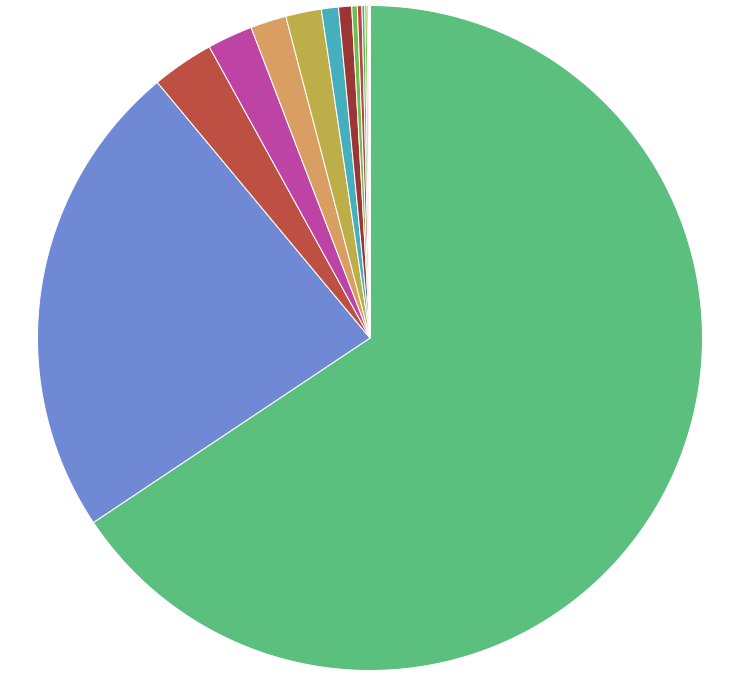
\includegraphics[height=2.5in]{comp-dunepro_pdsp_keepup.png}%
%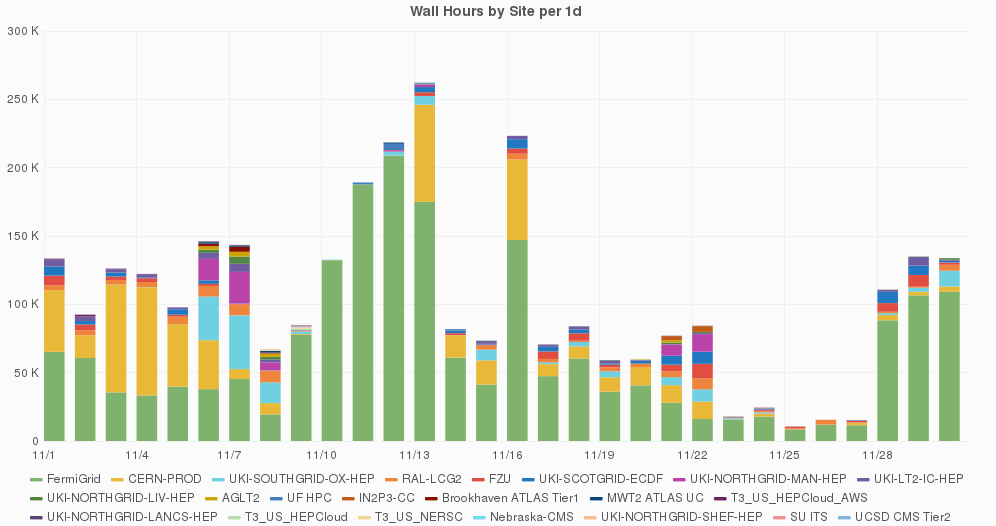
\includegraphics[height=4in]{comp-vo-summary}
%}
%\vspace{1cm}
%\subfloat[]{
%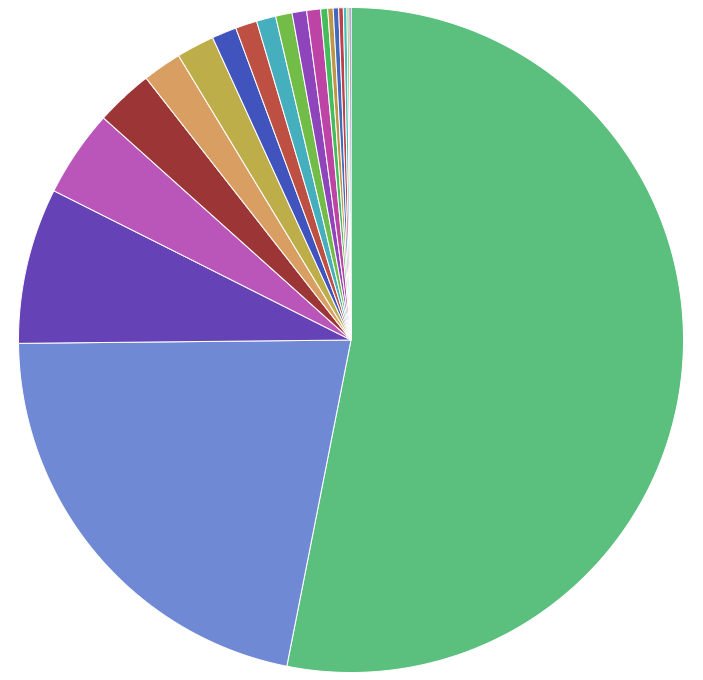
\includegraphics[height=2.3in]{comp-dunepro_mcc11.png}%
%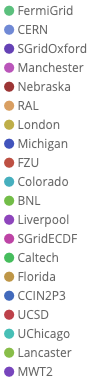
\includegraphics[height=2.3in]{comp-dunepro_mcc11_legend.png}
%}
\caption{CPU wall-time for November 2018 during ProtoDUNE-SP reconstruction showing multiple site contributions}
\label{fig:ch-exec-comp-cpupie}
\end{figure}
\fixme{comp-vo-summary.png was not found. Also, this should be structured as a dunefigure.}

\begin{dunetable}
[Data storage  and CPU needs for reconstruction of ProtoDUNE test beam data]
{llllll}{tab:exec-comp-needs}{Data storage and CPU needs for reconstruction of ProtoDUNE-SP test beam data taken in 2018}\\ \toprowrule
Detector& value &
2018&
2019&
2020&
2021\\  \colhline
&&As built&&&\\ \colhline

SP&
Events, M&
15.1&
13.0&
6.5&
40.5\\ \colhline
&
Raw data, TB&
1047&
2239&
1120&
2799\\ \colhline
&
Reco data, TB&
2094&
4479&
2239&
5599\\ \colhline
&
CPU, MH&
5.0&
4.3&
2.2&
13.5\\ \colhline

DP&
Events, M&
0.0&
101.1&
56.2&
119.9\\ \colhline
&
Raw data, TB&
0&
809&
449&
1799\\ \colhline
&
Reco data, TB&
0&
1617&
899&
3598\\ \colhline
&
CPU, MH&
0.0&
33.7&
18.7&
40.0\\
 \colhline
total&
Events, M&
15.1&
114.0&
62.6&
160.4\\ \colhline
&2x
Raw data, TB&
2094&
6096&
3138&
9197\\ \colhline
&
Reco data, TB&
2094&
6096&
3138&
9197\\ \colhline
&
CPU, MH&
5.0&
38.0&
20.9&
53.5\\ \colhline

total&Storage, TB &
4188&
12193&
6276&
18394\\
\end{dunetable}

\section{Lessons learned}

\begin{itemize}
    \item Data and simulation challenges led to a reasonably mature and robust model for acquiring, storing and cataloging the main data stream. 
    \item The experiment was able to integrate multiple existing grid sites and make use of substantial opportunistic resources.  This allowed initial processing of data within one month of the end of the run.
    \item Substantial but successful effort went into signal processing. 
    \item Reconstruction algorithms are not perfect but sufficient for studies of detector performance and calibration. 
    \item Beam information was successfully integrated into the processing through the \dword{ifbeam} database.
    \item Auxiliary information from, for example, slow controls was not integrated into processing due to lack of personpower.  This led to dependence on hand input of running conditions by shift personnel and offline incorporation of that information into the data catalog. 
\end{itemize}

Overall, the ProtoDUNE-SP data taking and processing was a success but overly dependent on doing things "by hand" as automated processes were not always in place. 






%%%%%%%%%%%%%%%%%%%%%%%%%%%%%%%%%%%%%%%%
\section{Evolving Data Model}		
\label{ch:exec-comp-mod}

%%%%%%%%%%%%%%%%%%%%
\subsection{Introduction}	
\label{ch:exec-comp-mod-int}
In parallel with the ProtoDUNE-SP data, a joint Data Model task force was formed by the DAQ and Computing Consortia. 

The Data Model task force grappled with the problems of efficiently triggering, reading out and storing data from an enormous detector on multiple time scales.

They defined major concepts.

\begin{description}

\item{Configuration:} set of parameters that define the persisted, expected detector state. Globally, this corresponds to a desirable state for the detector, capable of providing data of physics or calibration quality. Each component of the detector may have its own configuration.
 
\item{Run:} Period of time over which data has been collected across some set of desired components in a consistent configuration.
 
\item{Subrun:} Period of time within a run over which data has been collected across some set of desired components in a consistent configuration. The set of desired components in a subrun must be a subset of the desired components for a run, and is the set of components over which data is expected.
 
(Time-based rollovers of runs and subruns may be automatic. Differences of subrun and run due to configuration or changes in the desired components will be tracked by the DAQ, and may be either manual or automatic.)
 
\item{Trigger:} data from the desired components in that subrun over a window of time (a “readout window”). This would typically be centered around a trigger time, and is what is recorded by the DAQ. The readout window may be subdivided into “frames” as determined by the DAQ.
 
\item{Event:} subset of a trigger isolated in time and space containing an independent interaction in the detector. Events may overlap in space or time, within the same trigger. This is generally determined by the offline, based on reconstruction of data in a frame.

\end{description}

These definitions are intended to allow triggering, recording and reconstruction of interactions in subsets of the detector. While the whole detector (or time window) can produce enormous amounts of data, any individual interaction is expected to span a reasonably short time and spatial volume. A data model that can isolate individual interactions  allows efficient storage and reconstruction of interactions. 


The main data stream will be augmented by beam, slow controls, \dshort{daq} configuration and calibration information. 


\section{Consortium Organization}

The DUNE computing and software consortium was formed in October 2018.  
%%%%%%%%%%%%%%%%%%%%
%\subsection{Requirements}	
%\label{ch:exec-comp-mod-req}


%%%%%%%%%%%
%\subsubsection{How Physics Drives}
%\label{ch:exec-comp-mod-req-phys-drv}


%%%%%%%%%%%
%\subsubsection{Oscillation Analyses}
%\label{ch:exec-comp-mod-req-osc}


%%%%%%%%%%%
%\subsubsection{Cross Sections}
%\label{ch:exec-comp-mod-req-xsec}


%%%%%%%%%%%
%\subsubsection{Other Drivers}
%\label{ch:exec-comp-mod-req-oth-drv}


%%%%%%%%%%%%%%%%%%%%
%\subsection{Interfaces with Other Projects}	
%\label{ch:exec-comp-mod-intfc}


%%%%%%%%%%%
%\subsubsection{DAQ}
%\label{ch:exec-comp-mod-intfc-daq}


%%%%%%%%%%%
%\subsubsection{Calibration}
%\label{ch:exec-comp-mod-intfc-calib}

%Why is this cutting off here on the page?

%%%%%%%%%%%
%\subsubsection{Physics}
%\label{ch:exec-comp-mod-intfc-phys}

%Why is this cutting off here on the page?

%%%%%%%%%%%%%%%%%%%%
%\subsection{Use cases}	
%\label{ch:exec-comp-mod-use}


%%%%%%%%%%%
%\subsubsection{Discussion of detector options (SP,DP,ND… )}
%\label{ch:exec-comp-mod-use-opt}


%%%%%%%%%%%
%\subsubsection{Data acquisition}
%\label{ch:exec-comp-mod-use-daq}


%%%%%%%%%%%
%\subsubsection{Data Quality}
%\label{ch:exec-comp-mod-use-dq}


%%%%%%%%%%%
%\subsubsection{Reconstruction}
%\label{ch:exec-comp-mod-use-reco}


%%%%%%%%%%%
%\subsubsection{Calibration}
%\label{ch:exec-comp-mod-use-calib}


%%%%%%%%%%%
%\section{Simulation}
%\label{ch:exec-comp-mod-use-sim}


%%%%%%%%%%%
%\section{Analysis}
%\label{ch:exec-comp-mod-use-anls}


%%%%%%%%%%%%%%%%%%%%
%\subsection{Existing Infrastructure}	
%\label{ch:exec-comp-mod-infr}


%%%%%%%%%%%
%\subsubsection{sam/enstore/eos/castor}
%\label{ch:exec-comp-mod-infr-stor}


%%%%%%%%%%%
%\subsubsection{Grid}
%\label{ch:exec-comp-mod-infr-gr}


%%%%%%%%%%%
%\subsubsection{Databases}
%\label{ch:exec-comp-mod-infr-db}


%%%%%%%%%%%%%%%%%%%%
%\subsection{ProtoDUNE Experience}	
%\label{ch:exec-comp-mod-pdune}


%%%%%%%%%%%%%%%%%%%%
%\subsection{Evolving Infrastructure}	
%%\label{ch:exec-comp-mod-evlv}
%Why is this cutting off here on the page?

%%%%%%%%%%%
%\subsubsection{rucio}
%\label{ch:exec-comp-mod-evlv-ruc}
%Why is this cutting off here on the page?

%%%%%%%%%%%
%\subsubsection{Load Management}
%\label{ch:exec-comp-mod-evlv-load}


%%%%%%%%%%%
%\subsubsection{….}
%\label{ch:exec-comp-mod-evlv-}


%%%%%%%%%%%%%%%%%%%%
%\subsection{Novel Architectures}	
%\label{ch:exec-comp-mod-nov}

%%%%%%%%%%%
%\subsubsection{HPC}
%\label{ch:exec-comp-mod-nov-hpc}

%%%%%%%%%%%%%%%%%%%%
%\subsection{Authentication}	
%\label{ch:exec-comp-mod-auth}


%%%%%%%%%%%%%%%%%%%%%%%%%%%%%%%%%%%%%%%%
%\section{Software}		
%\label{ch:exec-comp-sw}


%%%%%%%%%%%%%%%%%%%%
%\subsection{Introduction}	
%\label{ch:exec-comp-sw-int}


%%%%%%%%%%%%%%%%%%%%
%\subsection{Existing Packages}	
%\label{ch:exec-comp-sw-int-pkg}


%%%%%%%%%%%
%\subsubsection{GEANT4}
%\label{ch:exec-comp-sw-int-gnt}


%%%%%%%%%%%
%\subsubsection{ROOT}
%\label{ch:exec-comp-sw-int-root}
%hy is this cutting off here on the page?

%%%%%%%%%%%
%\subsubsection{art}
%\label{ch:exec-comp-sw-int-art}


%%%%%%%%%%%%%%%%%%%%
%\subsection{Evolving Packages}	
%\label{ch:exec-comp-sw-evpkg}


%%%%%%%%%%%
%\subsubsection{LArSoft}
%\label{ch:exec-comp-sw-evpkg-larsoft}


%%%%%%%%%%%
%\subsubsection{Wirecell}
%\label{ch:exec-comp-sw-evpkg-wcell}


%%%%%%%%%%%
%\subsubsection{GENIE}
%\label{ch:exec-comp-sw-evpkg-genie}


%%%%%%%%%%%%%%%%%%%%
%\subsection{DUNE-specific Software}	
%\label{ch:exec-comp-sw-evpkg-spec}


%%%%%%%%%%%%%%%%%%%%
%\subsection{Novel Architectures}	
%\label{ch:exec-comp-sw-novarch}

%%%%%%%%%%%
%\subsubsection{Machine Learning}
%\label{ch:exec-comp-sw-novarch-mach}
%Why is this cutting off here on the page?
%%%%%%%%%%%
%\subsubsection{Vectorization}
%\label{ch:exec-comp-sw-novarch-vec}

%%%%%%%%%%%%%%%%%%%%
%\subsection{Development Environment	}
%\label{ch:exec-comp-sw-devenv}

%%%%%%%%%%%
%\subsubsection{Environment Specifications}
%\label{ch:exec-comp-sw-devenv-spec}


%%%%%%%%%%%
%\subsubsection{Code and Configuration Management}
%\label{ch:exec-comp-sw-devenv-mgmt}


%%%%%%%%%%%
%\subsubsection{Validation}
%\label{ch:exec-comp-sw-devenv-val}


%%%%%%%%%%%%%%%%%%%%
%\subsection{Training and Communication}	
%\label{ch:exec-comp-sw-train}
%Why is this cutting off here on the page?

%%%%%%%%%%%%%%%%%%%%
%\subsection{Lessons from ProtoDUNE}	
%\label{ch:exec-comp-sw-lessons}


%%%%%%%%%%%%%%%%%%%%%%%%%%%%%%%%%%%%%%%%
\section{Resources and Governance}		
\label{ch:exec-comp-gov}

The Computing and Software effort is now a DUNE Consortium.  Docdb 12751 \cite{bib:docdb12751} describes the governance structure for the Consortium.  The Consortium coordinates effort across the collaboration but funding comes from collaborating institutions, laboratories and national funding agencies. 

The consortium has an overall Consortium Leader. The Consortium Leader is responsible for the sub-system deliverables and represents the consortium to the overall DUNE collaboration.

In addition there  are Technical Leads to act as the overall project managers for the consortium. The Technical Leads report to the overall Consortium Leader.
Computing has both a Host Laboratory Technical Project Lead, responsible for coordination with the DUNE Project and host lab and an International Technical Lead responsible for coordination with institutions outside the US.

As with other DUNE consortia, the consortium is responsible for assigning a provisional division of institutional
responsibilities for computing resources, deliverables and operations, amongst the participating institutions. This division of responsibilities must account for the resources that are likely to be available. The internally agreed division of responsibilities needs to be presented to the Technical Board, which will then make a recommendation to the collaboration management for approval.



\subsection{Scope of the Consortium}
The Computing and Software Consortium  is mainly concerned with the infrastructure and resources for offline computing.  Algorithm development resides within the Physics groups while online systems at experimental sites are governed by the Data Acquisition and Cryogenics Instrumentation and Slow Controls Consortia. These groups coordinate closely to assure that the full chain of data acquisition, processing and analysis works. Formal interfaces with these groups are described in (DAQ)\cite{bib:docdb7123} and (CISC)\cite{bib:docdb7126}.

The consortium operates at two levels; at the hardware level, where generic resources can be provided as in kind contributions to the collaboration and at the human level, where individuals and groups contribute to the development of common software infrastructure. 

\subsection{Hardware}
As noted above, the collaboration has already made use of substantial global resources through the WLCG and OSG grid mechanisms. As the consortium evolves, institutions and collaborating nations will be asked to make formal pledges of resources (both CPU and storage) and those resources will be accounted for and considered in-kind contributions to the collaboration.
As illustrated above, several international partners are already making substantial contributions. We are currently integrating additional large national facilities. Most resources are currently opportunistic but Fermilab and CERN have committed several thousand cores and several PB of disk and the UK reserves 10\% of GridPP resources for non-LHC experiments, an allocation that DUNE has already benefited from.



\subsection{People}

The computing consortium has (or will have) subgroups for the following areas.  Highlights of some of the ongoing projects are detailed in subsequent sections. 

\begin{itemize}
    \item 
Collaborative Tools
\item Data Storage and Management
\item Databases 
\item Production and Processing 
\item Workflow Management
\item Data Quality Monitoring 
\item Software Release Management 
\item Core Software led by a Software Architect
\item Advanced Architectures
\item Algorithm liaisons
\item Networking
\end{itemize}
%%%%%%%%%%%%%%%%%%%%
\subsection{Cooperative Work with Other Collaborations	}
\label{ch:exec-comp-gov-coop}

\subsection{Relation to WLCG/OSG}
The WLCG has proposed a future governance structure that splits the dedicated resource provision for LHC experiments from the general middleware infrastructure used to access those resources.  This Scientific Computing Infrastructure (SCI) is already used by many other experiments worldwide.  In a white paper submitted to the European Strategy Group in December 2018\cite{SCI-EU}, a formal Scientific Computing Infrastructure organization is proposed. As part of the transition to that structure the DUNE collaboration has been provisionally invited to join the WLCG with observer status and participate in the Grid Management Board. The goal of our participation is to have input into the technical decisions on global computing infrastructure while contributing to that infrastructure. 

Areas of collaboration include

\subsection{rucio for Data Management}  %\dword{Rucio}  ``label'' wanted here?
\cite{rucio}
is a data management system originally developed by the ATLAS collaboration and now an open-source project.  DUNE has chosen to use Rucio for our large scale data movement.  In the short term it is being combined with the \dword{sam} data catalog used by Fermilab experiments.  DUNE collaborators at FNAL and in the UK are actively collaborating in the rucio project, adding value for DUNE but also the wider effort.

\begin{verbatim}
    

\end{verbatim}


%\todo{\verbatim{Add reference to http://wlcg-docs.web.cern.ch/wlcg-docs/technical_documents/HEP-Computing-Evolution.pdf}}

\todo{Text about LArsoft}

\subsection{Evaluations of other important infrastructure}

The DUNE S+C effort is still evaluating major infrastructure components, notably databases and workflow management systems.

For databases, the Fermilab Conditions Database is being used for the first run of protoDUNE but the Belle II\cite{https://docs.belle2.org/record/1192} system is also of interest. 

For workflow management, we are evaluating DIRAC \cite{DIRAC} and plan to investigate \cite{PandA}. Both of these systems are used by multiple LHC and non-LHC experiments and are being integrated with rucio. 

\fixme{i added Laycock:2019ynk to bib file. Anne}
\begin{verbatim}
\end{verbatim}



%%%%%%%%%%%%%%%%%%%%
%\subsection{Resource Needs}	
%\label{ch:exec-comp-gov-res}

%%%%%%%%%%%
%\subsubsection{Hardware}
%\label{ch:exec-comp-gov-res-hw}

%%%%%%%%%%%
%\subsubsection{Personnel}
%\label{ch:exec-comp-gov-res-hum}

%%%%%%%%%%%%%%%%%%%%
%\subsection{Contribution Models}	
%\label{ch:exec-comp-gov-contrib}
%Why is this cutting off here on the page?

%%%%%%%%%%%%%%%%%%%%
%\subsection{Technical Decision Governance}	
%\label{ch:exec-comp-gov-tech}

%%%%%%%%%%%%%%%%%%%%
%\subsection{Resource Decision Governance	}
%\label{ch:exec-comp-gov-resdec}

%%%%%%%%%%%%%%%%%%%%
%\subsection{Project Management}	
%\label{ch:exec-comp-gov-pm}


%%%%%%%%%%%%%%%%%%%%%%%%%%%%%%%  REMOVE THESE %%%%%%%%%%%%%
%\printglossaries
\end{document}
